% !TeX spellcheck = es_ES
\documentclass[a4paper,12pt]{article}
\usepackage[utf8]{inputenc}
\usepackage{graphicx}
\usepackage{float}
\usepackage{listings}
\usepackage{color}
\usepackage[spanish]{babel}
\usepackage[nottoc,notlot,notlof]{tocbibind} % Hace que se agregen las referencias al indice
 
\definecolor{codegreen}{rgb}{0,0.6,0}
\definecolor{codegray}{rgb}{0.5,0.5,0.5}
\definecolor{codepurple}{rgb}{0.58,0,0.82}
\definecolor{backcolour}{rgb}{0.95,0.95,0.92}
 
\lstdefinestyle{mystyle}{
    backgroundcolor=\color{backcolour},   
    commentstyle=\color{codegreen},
    keywordstyle=\color{magenta},
    numberstyle=\tiny\color{codegray},
    stringstyle=\color{codepurple},
    basicstyle=\footnotesize,
    breakatwhitespace=false,         
    breaklines=true,                 
    captionpos=b,                    
    keepspaces=true,                 
    numbers=left,                    
    numbersep=5pt,                  
    showspaces=false,                
    showstringspaces=false,
    showtabs=false,                  
    tabsize=2
}
 
\lstset{style=mystyle}

%opening
\title{Ejercicio del juego de la vida}
\author{Barrera Pérez Carlos Tonatihu \\ Profesor: Genaro Juárez Martínez \\ Computing Selected Topics \\ Grupo: 3CM8 }

\begin{document}

\maketitle
\newpage

\begin{figure}[H]
\begin{center}
 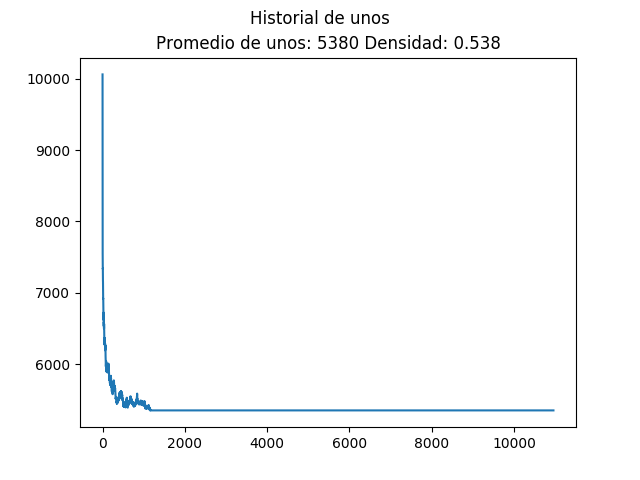
\includegraphics[width=12cm, height=7cm]{./quinientos.png}
 \caption{Matriz de 100x100 con 2000 iteraciones}
 \label{fig:diagrama}
\end{center}
\end{figure}

\begin{figure}[H]
\begin{center}
 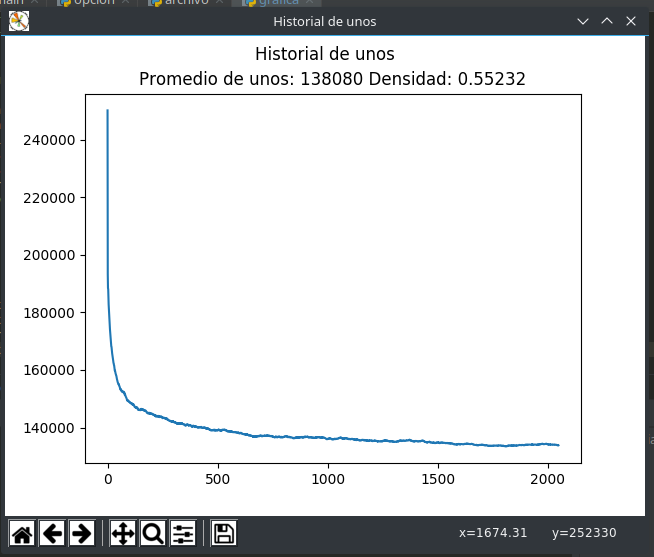
\includegraphics[width=12cm, height=7cm]{./cien.png}
 \caption{Matriz de 500x500 con 10000 iteraciones}
 \label{fig:diagrama}
\end{center}
\end{figure}

\end{document}
